\section{One decision depends on several versions}\label{sec:C17:state}
An agent's behavior depends on more than its model weights. The input view, memory store, retrieval index, tool schemas, harness, authorization, and environment each contribute to the conditional decision. Two runs using the same named model can implement different policies if any of these components changes. Conversely, identical stored text can produce different behavior when a new policy interprets it. Consistency is therefore a relation among components and transitions, not a property conferred by one database.

Define the complete system configuration at a decision boundary as
\begin{equation}
 Z_t=(H_t,\mathcal C_t,M_t,X_t,\theta_t,\delta_t,h_t,\mathcal T_t,A_t,\lambda_t,\nu_t,\alpha_t),
\end{equation}
where $H_t$ is recorded evidence, $\mathcal C_t$ the active view, $M_t$ memory, $X_t$ environment state, $\theta_t$ model parameters, $\delta_t$ deployment decoding, $h_t$ harness behavior, $\mathcal T_t$ tool contracts, $A_t$ trusted authority state, $\lambda_t$ the effect ledger, $\nu_t$ compatibility metadata, and $\alpha_t$ the current authority epoch. Not every component is fully observable, particularly the external environment and proprietary model implementation. A consistency claim must state which components it constrains and which remain outside the guarantee.

Let $g_{\nu,h}$ be the versioned context-assembly map, including selection and serialization. Any random assembly choices are retained as decision evidence or as a materialized view, rather than assumed recoverable from a seed alone. Let $A_t^{\rm vis}$ be the policy-safe projection of authority; the trusted monitor can retain more privileged information. The request is part of $H_t$. The deployed proposal law is
\begin{equation}
 \mathcal C_t=g_{\nu_t,h_t}(H_t,M_t,\mathcal T_t,A_t^{\rm vis}),
 \qquad P(a_t\mid Z_t)=\Pi_{\theta_t,\delta_t,h_t}(a_t\mid\mathcal C_t,\mathcal T_t),
\end{equation}
followed by a current-authority enforcement and execution transition. The law includes the parser and stopping semantics of Chapter~\ref{ch:C02}. Governing implementations remain fixed within a comparison epoch; selecting a versioned skill or editing its runtime input can change state without changing its interpreter. A changed executable resource or model checkpoint requires an explicit configuration transition. Restoring $\nu_t$ cannot restore an expired grant or revise $\lambda_t$ without new effect evidence. This formulation is original synthesis. It makes explicit that assembly and monitoring can change behavior without a weight update. It also identifies why a model-only benchmark cannot certify a complete deployed agent.

Consistency has several meanings. Conditioning consistency preserves what was visible when an action was sampled. Semantic consistency preserves the status and scope of assertions across memory transformations. Transactional consistency governs concurrent reads and writes. Computational consistency governs whether cached states correspond to the input being evaluated. Authority consistency preserves the current allowed-action boundary. These properties interact but are not equivalent; satisfying one should not be described as satisfying all.

The three contracts in Chapter~\ref{ch:C01} provide a common test across those mechanisms. Proposal preservation constrains the distribution produced from a transformed view. Authority nonexpansion constrains the admissible effects, even when proposals change. Effect-state preservation constrains the ledger needed to distinguish pending, committed, and reconciled operations. Conditioning consistency adds a training obligation: an unchanged terminal artifact cannot justify assigning an earlier action a history it never saw. Thus a context edit can preserve authority and effect records while changing proposals, and a perfect behavior replay can still be invalid under revoked authority. The component checks need to identify which contract they establish.

The 2026 context-management literature provides concrete instances. MemoryWalker examines rollout and training views~\cite{j2026memorywalker}; CLM couples editable context with serving behavior~\cite{shao2026context}; HyperSkill changes reusable memory while retaining a task-level retrieved context~\cite{xu2026hyperskill}. Their mechanisms occupy different transitions in $Z_t$. A coherent architecture must specify how those transitions compose rather than assuming that each component's local improvement remains beneficial after integration.


% SCIENTIFIC_FIGURE_C17
Figure~\ref{fig:C17:overview} compares action laws under a fixed deployment and different views of common recorded history.
\begin{figure}[!htbp]
\centering
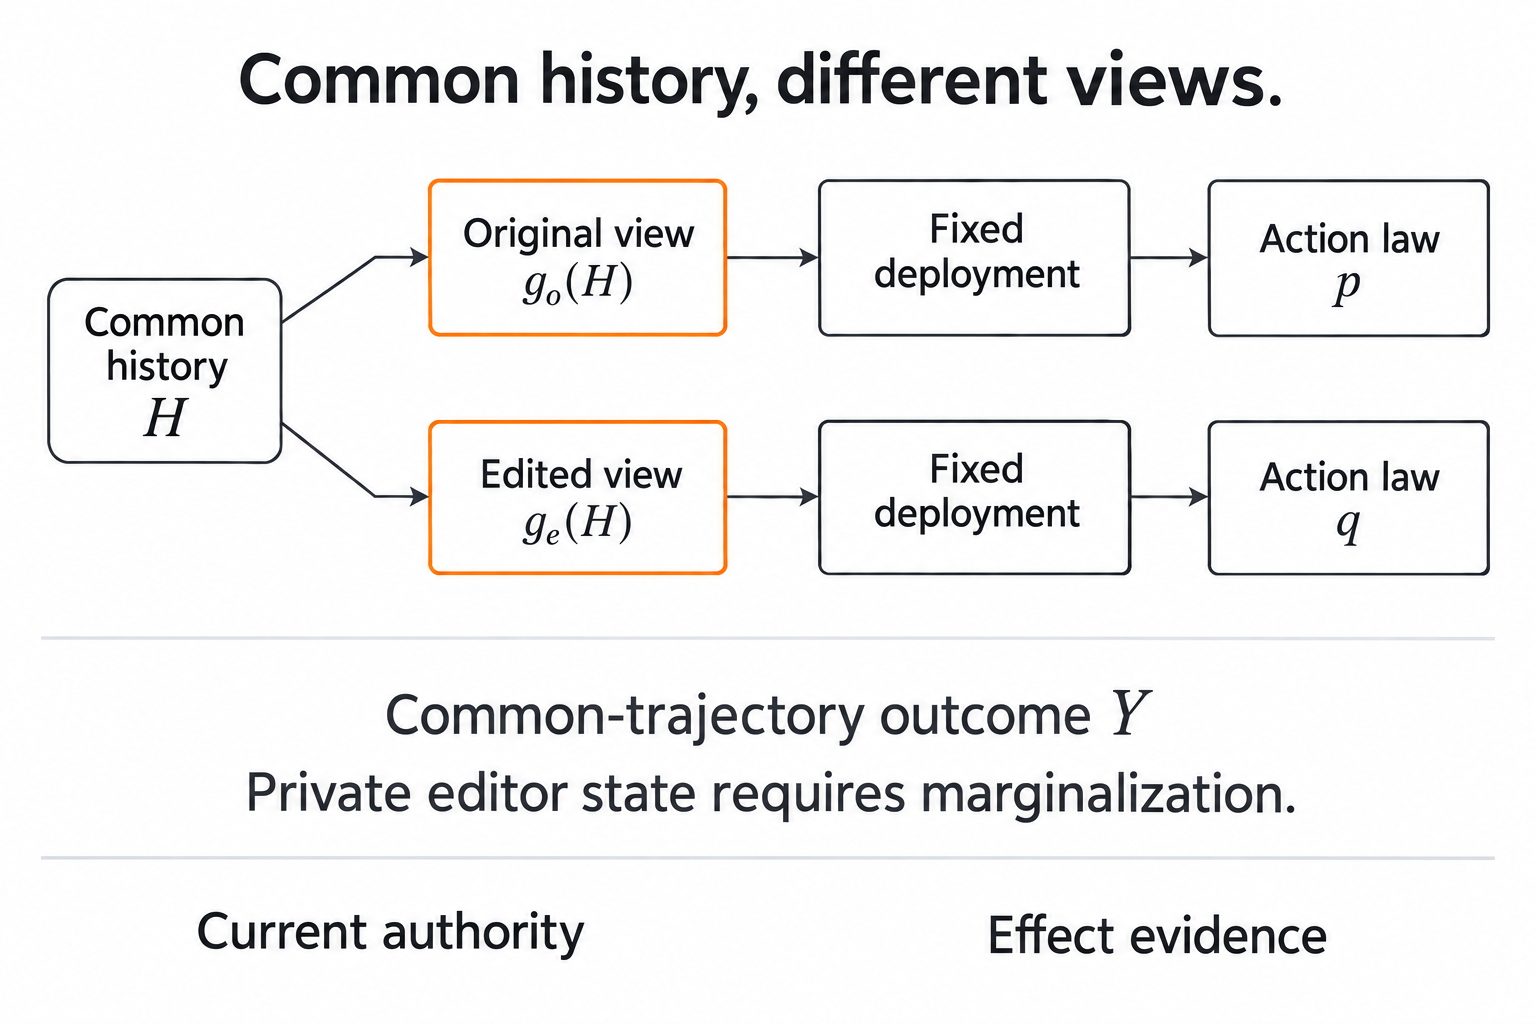
\includegraphics[width=\linewidth]{book/figures/assets/F17review.png}
\caption{Different deterministic views of common permitted recorded history $H$ can induce different action laws $p,q$ under one fixed deployment. Model/tokenizer, decoder, parser and decision interface are held fixed. The behavioral bound concerns outcomes $Y$ on the common trajectory; random private editor state requires conditional marginalization. Two sampled prompts do not establish that premise. Current authority and effect evidence remain independent checks.}
\label{fig:C17:overview}
\end{figure}
